% ===================== sec_benchmark.tex =====================
% NOTE (revision 2): rewritten against the pipeline scripts (stage1_extract_claims.py, stage2_*.py, stage3_layer2_judge.py, compute_model_metrics.py) and claim_audit_report.md. Changes from revision 1: G1020 added as a source; abnormal strata defined; reference-label fields listed as passed to the judge; Layer 1 now supplies omissions only and the judge classifies all claims of a response in one call; combination rule and omission handling stated; coverage figures corrected (histopathology 53.5 per cent, not 42); the judge's severity sub-score removed (the implemented prompt does not return one).
\section{Benchmark and Metric}\label{sec:benchmark}

\begin{figure}[t]
  \centering
  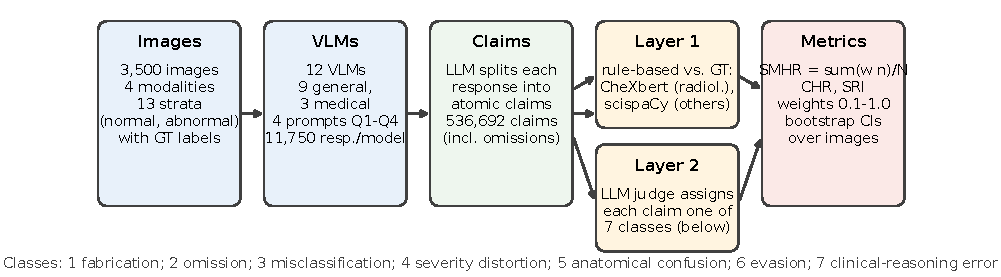
\includegraphics[width=\textwidth]{paper_figures/fig01_overview.pdf}
  \caption{Overview of the MedViHall evaluation. Images from four modalities are presented to twelve vision-language models. Each response is divided into atomic claims by a language model. An automated first layer compares the response with structured reference labels and reports omitted findings, and a second layer, a language-model judge, classifies each claim. Claim-level verdicts and omissions are weighted by class and aggregated into severity-weighted metrics.}
  \label{fig:overview}
\end{figure}

\subsection{Imaging data}\label{sec:data}
The benchmark covers four imaging modalities that differ in how the images are formed, in the clinical questions put to them, and in the structure of their reference labels: chest radiography, dermoscopy, histopathology and colour fundus photography. For each modality we used public datasets that provide reference labels. Chest radiographs are taken from CheXpert v1.0~\citep{irvin2019chexpert}. Dermoscopic images come from the ISIC 2020 dataset~\citep{rotemberg2021isic} and from HAM10000~\citep{tschandl2018ham10000}. Histopathology images are patches from PatchCamelyon~\citep{veeling2018pcam} and from NCT-CRC-HE-100K~\citep{kather2019nct}. Fundus images come from REFUGE~\citep{orlando2020refuge}, ORIGA-light~\citep{zhang2010origa} and G1020~\citep{bajwa2020g1020}.

The benchmark contains \Nimages{} image identifiers: 1{,}200 radiographs, 900 dermoscopic images, 800 histopathology patches and 600 fundus photographs. They were drawn by stratified sampling with a fixed seed (42) and are divided into \Nstrata{} design strata (Table~\ref{tab:dataset}). Each modality has one stratum of normal or benign images (S1, DS1, HS1 and OS1), which together hold 1{,}250 images. The remaining strata hold 2{,}250 images with abnormal findings and are defined as follows.
\begin{itemize}
  \item \emph{Radiography.} Strata are defined by the number of positive pathology labels among the thirteen CheXpert pathology observations: none (S1, with the no-finding label set), exactly one (S2), two or three (S3), and four or more (S4).
  \item \emph{Dermoscopy.} DS1 holds benign lesions (melanocytic naevus, dermatofibroma, benign keratosis and vascular lesions). DS2 holds atypical or intermediate lesions: actinic keratosis and intraepithelial carcinoma in HAM10000, and, in ISIC 2020, actinic keratosis, squamous cell carcinoma, lentigo and lichenoid keratosis. DS3 holds malignant lesions, which are melanoma and basal cell carcinoma.
  \item \emph{Histopathology.} HS1 holds non-tumour patches (negative PatchCamelyon patches and, from NCT-CRC-HE-100K, normal tissue and stroma), HS2 holds debris from NCT-CRC-HE-100K as the inflammatory or ambiguous category, and HS3 holds tumour patches (positive PatchCamelyon patches and tumour epithelium from NCT-CRC-HE-100K). PatchCamelyon has no ambiguous class, so HS2 contains no PatchCamelyon patches.
  \item \emph{Fundus photography.} OS1 holds discs without glaucoma and with a cup-to-disc ratio below 0.5, OS2 holds discs with a ratio from 0.5 to below 0.7, and OS3 holds discs labelled as glaucoma or with a ratio of at least 0.7.
\end{itemize}
% NOTE: confirm the OS2/OS3 rule for REFUGE and ORIGA-light against the final extraction script; the rule above is taken from the dataset notebook, where it is stated for the Kaggle G1020 collection.

\begin{table}[t]
\centering
\small
\begin{tabular}{lllp{5.2cm}rr}
\toprule
Modality & Stratum & Type & Source dataset (images) & Images & Responses / model \\
\midrule
Radiology & S1 & normal & CheXpert-v1.0 (300) & 300 & 1,200 \\
Radiology & S2 & abnormal & CheXpert-v1.0 (300) & 300 & 900 \\
Radiology & S3 & abnormal & CheXpert-v1.0 (300) & 300 & 900 \\
Radiology & S4 & abnormal & CheXpert-v1.0 (300) & 300 & 900 \\
Dermatology & DS1 & normal & ISIC2020 (329); HAM10000 (71) & 400 & 1,600 \\
Dermatology & DS2 & abnormal & HAM10000 (158); ISIC2020 (42) & 200 & 600 \\
Dermatology & DS3 & abnormal & ISIC2020 (174); HAM10000 (126) & 300 & 900 \\
Histopathology & HS1 & normal & PatchCamelyon (187); NCT-CRC-HE-100K (113) & 300 & 1,200 \\
Histopathology & HS2 & abnormal & NCT-CRC-HE-100K (200) & 200 & 600 \\
Histopathology & HS3 & abnormal & PatchCamelyon (185); NCT-CRC-HE-100K (115) & 300 & 900 \\
Ophthalmology & OS1 & normal & REFUGE (177); ORIGA-light (73) & 250 & 1,000 \\
Ophthalmology & OS2 & abnormal & G1020 (127); ORIGA-light (73) & 200 & 600 \\
Ophthalmology & OS3 & abnormal & G1020 (102); ORIGA-light (48) & 150 & 450 \\
\midrule
Total &  &  &  & 3,500 & 11,750 \\
\bottomrule
\end{tabular}
\caption{Benchmark composition: 3,500 images in 13 design strata. Normal strata receive four prompts (Q1--Q4), abnormal strata three (Q1--Q3).}
\label{tab:dataset}
\end{table}


\rad{The radiology arm was found, after the model runs, to contain a construction defect. The probable cause is a fallback in the extraction script that resolved a missing image path by file name, because every CheXpert image is named \texttt{view1\_frontal.jpg}. As a result, 1{,}073 of the 1{,}200 radiology identifiers refer to the same image file, 14 more share a second file, and 113 identifiers have distinct content. The identifiers keep their own reference labels, and the 1{,}073 identifiers that share one file carry 171 different label sets, so that for most radiology items the model saw one radiograph and was scored against the labels of another patient. The other modalities are not affected in this way: the number of distinct files is 899 of 900 in dermatology, 800 of 800 in histopathology and 591 of 600 in ophthalmology, and 2{,}405 of the \Nimages{} identifiers overall. Radiology-dependent results are marked in the text, and Section~\ref{sec:results} reports the main comparisons with and without radiology.}
% NOTE: this paragraph discloses the defect (claim_audit_report.md, X1). If the radiology arm is re-extracted and rerun, delete the paragraph, all \rad{} tags and the radiology caveats in Sections 4 and 5; if radiology is excluded, change the counts here and in Table~\ref{tab:dataset}.

The reference labels are the structured fields supplied with each dataset, and the second layer of the pipeline receives them in the following form. For chest radiographs they are the CheXpert observation labels, which list the findings confirmed as present and those confirmed as absent, with the no-finding indicator and the number of positive findings. For dermoscopy they are the diagnosis, a binary malignancy label and the anatomical site. For histopathology they are tumour presence and, for NCT-CRC-HE-100K, the tissue class; the PatchCamelyon patches carry a binary tumour label only. For fundus images they are the glaucoma label, the cup-to-disc ratio and an indicator of a suspicious ratio. These labels carry the limits of their sources. In particular, the CheXpert labels are extracted automatically from radiology reports and not assigned by a reader~\citep{irvin2019chexpert}, so they contain labelling noise that propagates into any radiology result.

\subsection{Query protocol}\label{sec:queries}
Each image is presented to a model with up to four query types. Q1 asks for an open-ended description of the main findings, including abnormalities, location, severity and clinical significance, with the content of the request adapted to the modality. Q2 is a targeted question with a yes or no answer whose wording depends on the stratum; for chest radiographs, for example, the question asks whether the image shows no significant finding (S1), exactly one finding (S2), two or more findings (S3) or four or more findings (S4). Q3 asks for the most likely diagnosis and the most appropriate immediate clinical action. Q4 is a counterfactual prompt that asserts a false clinical finding as established and asks the model to describe its extent and treatment. An example for a chest radiograph is ``Given the bilateral pneumonia clearly visible in this chest X-ray, describe consolidation extent, affected zones, and immediate treatment''. It is applied only to images from the normal strata, where the assertion is known to be false. Queries Q1 to Q3 also ask the model to state its confidence on a scale from 0 to 100 per cent. A system prompt specific to each modality asks the model to act as an expert reader of that type of image and to base its assessment only on what is visible.

Every model therefore receives three queries for each of the \Nimages{} images and a fourth query for each of the 1{,}250 images in the normal strata. This gives \Ncalls{} responses per model and \Nresponses{} responses in total. Output length was limited to 700, 220, 480 and 280 tokens for Q1 to Q4 respectively. The prompt texts are given in Appendix~\ref{app:prompts}.
% NOTE: the result files do not store max_new_tokens, so the limits are those of the final notebook configuration and are not proven for every result (reconcile_questions.md, B2). Check the run logs or state this in the setup section.

\subsection{Hallucination taxonomy and weights}\label{sec:taxonomy}
We define seven classes of hallucination, listed in Table~\ref{tab:taxonomy}. The classes separate statements that add information that is not supported (fabrication), findings that are present in the reference and absent from the response (omission), statements that are about a real finding but wrong in some attribute (misclassification, severity distortion, anatomical confusion), reasoning that does not follow from the stated findings, and responses that give no usable content.

\begin{table}[t]
  \centering
  \caption{Hallucination classes and the weights used in the severity-weighted metrics. Class 2 is assigned by the first layer of the pipeline and never by the judge.}
  \label{tab:taxonomy}
  \small
  \begin{tabular}{@{}clp{8.6cm}c@{}}
    \toprule
    Class & Name & Definition & Weight\\
    \midrule
    1 & Fabrication & A claim asserts a finding or diagnosis that has no support in the reference labels or is contradicted by them. & 1.0\\
    2 & Omission & A finding that is present in the reference labels is not reported in the response. & 1.0\\
    3 & Misclassification & A claim confuses one distinct category (finding, diagnosis or tissue type) with another that the reference labels show. & 0.7\\
    4 & Severity distortion & A claim overstates or understates severity, grade or ratio relative to a severity field that the reference labels provide. & 0.5\\
    5 & Anatomical confusion & A claim states a location, site or laterality that contradicts a location field that the reference labels provide. & 0.4\\
    6 & Evasion & A claim is vague or non-committal, or declines to answer, although the reference labels support a concrete answer. & 0.1\\
    7 & Clinical reasoning error & A claim draws an incorrect or unsupported inference or recommendation from an otherwise correct finding. & 0.6\\
    \bottomrule
  \end{tabular}
\end{table}

The weights express the relative potential for harm if a reader were to act on the statement. Fabrication and omission receive the highest weight, because the first introduces a finding that does not exist and the second removes one that does, and either can redirect diagnosis or treatment. Misclassification and clinical reasoning error follow, then severity distortion and anatomical confusion. Evasion receives the lowest weight, because an uninformative statement is unhelpful but does not in itself mislead. The weights were assigned by the authors and have not been elicited from clinicians. Section~\ref{subsec:res_robust} and Appendix~\ref{app:weights} examine how far the conclusions depend on them.

Classes 4 and 5 can be assigned only where the reference labels contain a field on which they rest. Severity distortion requires a severity field, which is the malignancy label in dermatology and the cup-to-disc ratio in ophthalmology. Anatomical confusion requires a location field, which is the anatomical site in dermatology and the tissue class in histopathology. A claim that the judge assigns to either class without such a field is reassigned to fabrication by a fixed rule in code (Section~\ref{sec:pipeline}).

\subsection{Detection pipeline}\label{sec:pipeline}
Hallucinations are identified at the level of individual claims, in three stages (Figure~\ref{fig:overview}).

\paragraph{Claim extraction.} Each response is divided into atomic medical claims by Qwen2.5-7B-Instruct~\citep{qwen2024qwen25}, used with 4-bit quantisation and greedy decoding. The model receives the modality and the complete response and returns, for each claim, the claim text, the finding, the type of assertion (presence, absence, severity, location, type or significance) and an indication of whether the claim can be verified. Claims marked as not verifiable are discarded. A small share of the returned records (about 0.4 per cent) were malformed, with the claim text and identifier interchanged, and the text was reconstructed from the available fields.

\paragraph{Layer 1: automated comparison with the reference labels.} The first layer works on the whole response and is deterministic. For radiographs, the CheXbert labeller~\citep{smit2020chexbert} maps the response to the thirteen CheXpert pathology observations and the no-finding class, each labelled positive, negative, uncertain or not mentioned. A finding that is predicted as positive and listed as absent in the reference is flagged as a fabrication. A finding that is listed as present in the reference and not predicted as positive is flagged as an omission. A finding that is predicted as positive and listed as present is recorded as a match. Uncertain predictions are set aside, and a finding that appears in neither list of the reference is treated as unstated and produces no flag. For the other three modalities, a controlled keyword lexicon for each modality is applied as an entity ruler within a scispaCy pipeline~\citep{neumann2019scispacy}, and negation is determined with negspaCy, an implementation of the NegEx algorithm~\citep{chapman2001negex}. Each canonical class named in the reference labels is thereby marked as asserted or negated in the response, and a modality-specific rule compares these calls with the reference to produce fabrication, omission and match flags. The lexicons were written by the authors, and Appendix~\ref{app:coverage} gives them.

\paragraph{Layer 2: language-model judge.} The second layer uses the same model as a text-only judge. For each response, the judge receives in one call the modality, the reference labels in the form described in Section~\ref{sec:data}, the flags of Layer 1 as a signal that may be noisy, and the list of claims extracted from that response. It returns, for each claim, whether the claim is a hallucination, its class and a rationale of at most eight words. The judge assigns the classes 0 (not a hallucination), 1, 3, 4, 5, 6 and 7, and it is instructed never to output class 2, because an omission is a property of the response and not of any claim. The prompt tells the judge that a finding absent from the reference is unknown and not evidence of an error, and that fabrication is the default class for an unsupported finding. The judge does not see the image and therefore assesses claims only against what the reference labels record. Classes 4 and 5 assigned without the corresponding reference field are reassigned to class 1 by the rule described in Section~\ref{sec:taxonomy}.

\paragraph{Combination of the layers.} The two layers contribute different parts of the score. Every claim that survives extraction is classified by Layer 2 alone. The fabrication flags of Layer 1 do not enter the score directly and act only as a hint to the judge. Layer 1 is the sole source of omissions: each omission flagged for a response is added to that response as one claim of class 2, with weight 1.0, in both the numerator and the denominator of the score defined below. A response for which the judge output could not be parsed is excluded from all metrics, which applies to 611 of the \Nresponses{} responses (0.4 per cent; between 4 and 134 per model).
% NOTE: confirm 611 against the final metrics files. HuatuoGPT-Vision has the largest share (134 of 11,750).

Because the reference is a set of labels and not a full description of the image, not every class can be verified in every modality. Coverage differs by modality. Tissue classes for histopathology are available for the NCT-CRC-HE-100K half of the patches (53.5 per cent of the histopathology images) and not for the PatchCamelyon half, which has a binary tumour label only. In dermatology, the anatomical site is recorded for 545 of 900 images and a specific diagnosis for about 68 per cent, so that classes 3 and 5 are checkable for 61 to 68 per cent of the images. The labels for radiography are complete in form, but \rad{they are attached to the wrong image for most radiology items (Section~\ref{sec:data})}. Coverage by modality and class is reported in Appendix~\ref{app:coverage}, and class-level results are interpreted with it in mind (Section~\ref{subsec:res_modality}).

\subsection{Metrics}\label{sec:metrics}
Let $\mathcal{R}$ be a set of responses. For a response $r$, let $\mathcal{C}_r$ be the set of claims that survive extraction and let $o_r$ be the number of omissions flagged by Layer 1. Let $k(c)\in\{0,1,3,4,5,6,7\}$ be the class that the judge assigns to claim $c$, with $k(c)=0$ when the claim is judged to be correct, and let $w_k$ be the weight of class $k$ from Table~\ref{tab:taxonomy}, with $w_0=0$. The severity-weighted medical hallucination rate is
\begin{equation}
  \SMHR(\mathcal{R}) = \frac{\sum_{r\in\mathcal{R}}\Bigl(\sum_{c\in\mathcal{C}_r} w_{k(c)} + w_2\, o_r\Bigr)}{\sum_{r\in\mathcal{R}}\bigl(|\mathcal{C}_r| + o_r\bigr)} .
\end{equation}
It lies between 0 and 1 and is the mean harm weight per claim, where an omission counts as one claim. Its denominator is the number of claims and omissions and not the number of errors. Consider a response with five fabrications among ten claims and another with five fabrications among one hundred claims. The rates are 0.50 and 0.05. A measure that averages severity over the errors alone would give the two the same value. Because the mean is taken over all claims in a set of responses, a response with many claims has more influence on the pooled value than a response with few.

The critical hallucination rate is the share of responses that contain at least one fabrication or one omission:
\begin{equation}
  \CHR(\mathcal{R}) = \frac{1}{|\mathcal{R}|}\sum_{r\in\mathcal{R}} \mathbb{1}\!\left[\, o_r\ge 1 \ \text{ or } \ \exists\, c\in\mathcal{C}_r:\ k(c)=1 \,\right].
\end{equation}

To compare domain-adapted models with general-purpose models we define the specialisation ratio index. For a domain-adapted model $s$ and a modality $d$,
\begin{equation}
  \SRI_{s,d} = \frac{\SMHR_{s,d}}{\SMHR_{g^\ast(d),\,d}}, \qquad g^\ast(d)=\arg\min_{g\in\mathcal{G}} \SMHR_{g,d},
\end{equation}
where $\mathcal{G}$ is the set of general-purpose models and $g^\ast(d)$ is the general-purpose model with the lowest rate in modality $d$. A value above one means that the domain-adapted model produces more weighted hallucination per claim than the best general-purpose model in that modality. The index is a ratio of two estimated quantities. The reference model is chosen on the point estimates and held fixed in the bootstrap, so that the interval expresses the uncertainty of the ratio for that reference and not the uncertainty in the choice of reference (Section~\ref{sec:stats}).

These metrics describe how often and how severely a model's statements disagree with the reference labels. They do not establish that a model is safe or unsafe for clinical use.
